\documentclass[11pt, xcolor={dvipsnames}, hyperref={colorlinks, allcolors=Blue}]{beamer}


% Packages
\usepackage{graphicx}
\usepackage{caption, subcaption}
\usepackage{tikz}
\usepackage{amsmath, amsfonts, amssymb}
\usepackage{bm}
\usepackage{booktabs}
\usepackage{apacite}
\usepackage{multirow}
\usepackage{multicol}
\usepackage{doi}
\usepackage{textpos}
\usepackage{lipsum}
\usepackage{amsfonts, amsmath}
\usepackage{wrapfig}
\usepackage{animate}
\usepackage{cleveref}


\renewcommand\doiprefix{}


\usepackage{tikz}
\usetikzlibrary{shapes, fit}





%%%%%%%%%%%%%%%%%%%%%%%%%%%%%%%%%%%%%%%%%%%%%%
% Custom commands
\newcommand\bc[1]{{\usebeamercolor[fg]{frametitle} {\textbf{#1}}}} % bold and color
\newcommand{\into}{\rightarrow}



%%%%%%%%%%%%%%%%%%%%%%%%%%%%%%%%%%%%%%%%%%%%%%
% Set Theme
\usetheme{Boadilla}
\usecolortheme{rose}

%%%%%%%%%%%%%%%%%%%%%%%%%%%%%%%%%%%%%%%%%%%%%%
% Make citation font tiny
\renewcommand{\bibliographytypesize}{\tiny}

%%%%%%%%%%%%%%%%%%%%%%%%%%%%%%%%%%%%%%%%%%%%%%
% Fonts
\usefonttheme{serif} % Serif font
\setbeamertemplate{enumerate items}[default] % Don't use bullets in enumerate.

%%%%%%%%%%%%%%%%%%%%%%%%%%%%%%%%%%%%%%%%%%%%%%%
% Remove navigation bar
\setbeamertemplate{navigation symbols}{}
%%%%%%%%%%%%%%%%%%%%%%%%%%%%%%%%%%%%%%%%%%%%%%


% Frontmatter
\title[ECON 8000 -  Lecture 7]{Lecture 7: Calculus}
\author[University of Queensland]{Robert Garrard}
\date[\today]{} 


%%%%%%%%%%%%%%%%%%%%%%%%%%%%%%%

% Common commands

% Sets
\newcommand{\R}{\mathbb{R}}
\newcommand{\N}{\mathbb{N}}
\newcommand{\Z}{\mathbb{Z}}
\newcommand{\Q}{\mathbb{Q}}
\renewcommand{\P}{\mathbb{P}}
\newcommand{\E}{\mathbb{E}}

% Symbols
\renewcommand{\epsilon}{\varepsilon}
\renewcommand{\implies}{\Rightarrow}
\newcommand{\halmos}{\hfill$\blacksquare$}

% Vector notation
\renewcommand{\a}{\mathbf{a}}
\renewcommand{\b}{\mathbf{b}}
\newcommand{\h}{\mathbf{h}}
\newcommand{\x}{\mathbf{x}}
\newcommand{\X}{\mathbf{X}}
\newcommand{\y}{\mathbf{y}}
\newcommand{\z}{\mathbf{z}}
\renewcommand{\v}{\mathbf{v}}
\newcommand{\bepsilon}{\mathbf{\varepsilon}}
\newcommand{\bbeta}{\mathbf{\beta}}

% Matrices
\newcommand{\eyetwo}{\begin{pmatrix} 1 & 0\\ 0 & 1 \\ \end{pmatrix}} % I_2 identity matrix
\newcommand{\eyethree}{\begin{pmatrix} 1 & 0 & 0\\ 0 & 1 & 0\\ 0 & 0 & 1 \end{pmatrix}} % I_3 identity matrix
\newcommand{\zerotwo}{\begin{pmatrix} 0 & 0\\ 0 & 0 \\ \end{pmatrix}} % 2x2 Zero matrix
\newcommand{\zerothree}{\begin{pmatrix} 0 & 0 & 0\\ 0 & 0 & 0\\ 0 & 0 & 0 \end{pmatrix}} % 3x3 Zero matrix


% Misc

\newcommand{\innerprod}[2]{\langle #1, #2 \rangle}


%%%%%%%%%%%%%%%%%%%%%%%%%%%%%%%%

% Tikz
\usetikzlibrary{arrows,shapes,trees, positioning}

%%%%%%%%%%%%%%%%%%%%%%%%%%%%%%

\newcounter{Lecture}
\addtocounter{Lecture}{7}

\newcounter{exercise}
\newenvironment{exercise}[1][]{\refstepcounter{exercise}\par\medskip
   \noindent {\bc{Exercise}~\bc{\theLecture.\theexercise} #1}}{\medskip}


\begin{document}

\begin{frame}
\titlepage

%\begin{picture}(0,0)
%\put(35,-50){\hbox{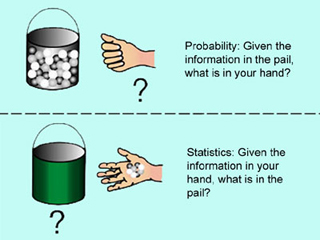
\includegraphics[width=0.8\textwidth, trim={0cm, 1cm, 0cm, 1cm}, clip]{prob_stats}}}
%\end{picture}

\end{frame}
%%%%%%%%%%%%%%%%%%%%%%%%%%%%%%%%%%%%%%%%%%%%%%%
\begin{frame}{Taylor Series}
There is a class of functions, called \bc{analytic functions}, which have a very special property.\bigskip

 In a neighbourhood of some point, the function is described by a convergent power series.\bigskip

 Examples of analytic functions include all polynomials, the exponential and logarithm functions, trigonometric functions, and power functions. \bigskip


Let $f:\R\into\R$ be an infinitely differentiable function. The \bc{Taylor series} about some point $a\in\R$ is the power series

\[f(x) = \sum_{n = 0}^{\infty} \frac{f^{(n)}(a)}{n!}\left(x-a\right)^{n}\]


\end{frame}

%%%%%%%%%%%%%%%%%%%%%%%%%%%%%%%%%%%%%%%%%%%%%%%
\begin{frame}{Taylor Series}
\begin{block}{Example}
Determine the Taylor series about $a=0$ for the function 
\[f:\R\into\R \quad \quad f(x) = e^{x}\]

Since the derivative of the exponential function is itself, $f^{(n)}(x) = e^{x}$. The $n$th derivative about $a=0$ is therefore $e^{0} = 1$.	The Taylor series for $e^{x}$ about zero is 

\[e^{x} = \sum_{n=0}^{\infty} \frac{x^{n}}{n!}\]
\[ = 1 + x + \frac{x^{2}}{2} + \frac{x^{3}}{6} + \frac{x^{4}}{24}...\]

\end{block}

\end{frame}

%%%%%%%%%%%%%%%%%%%%%%%%%%%%%%%%%%%%%%%%%%%%%%%
\begin{frame}{Taylor Series}
\begin{figure}
	\centering
	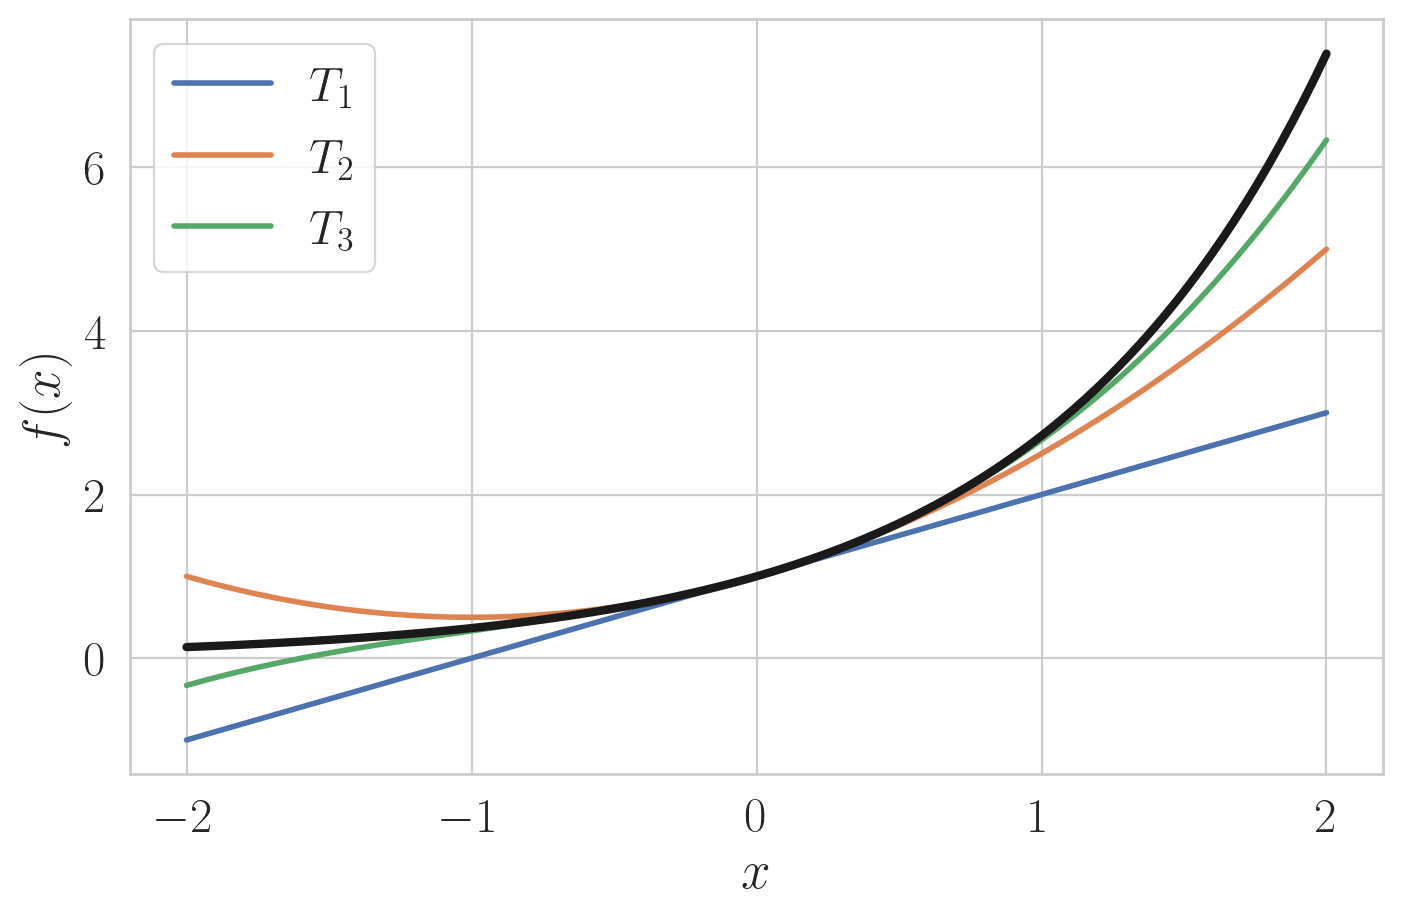
\includegraphics[width=0.75\textwidth]{taylor_e.png}
	\caption{3 Taylor polynomials of $e^{x}$}
\end{figure}

\end{frame}

%%%%%%%%%%%%%%%%%%%%%%%%%%%%%%%%%%%%%%%%%%%%%%%
\begin{frame}{Taylor Series}
\begin{exercise}
Find the Taylor expansion of $f(x) = \log(1+x)$ about $x=0$.
\end{exercise}
\bigskip\vfill\bigskip\vfill
\end{frame}

%%%%%%%%%%%%%%%%%%%%%%%%%%%%%%%%%%%%%%%%%%%%%%%
\begin{frame}{Taylor Series}

\begin{theorem}
Let $f:\R\into\R$ be $k$ times differentiable at the point $a\in\R$. Then there exists a function $R_{k}:\R\into\R$ such that

\[f(x) = f(a) + f^{'}(a)\left (x-a\right) + \frac{f^{''}(a)}{2}\left(x-a\right)^{2} + \dots + \frac{f^{(k)}}{k!} \left(x-a\right)^{k} + R_{k}(x)\]
such that
\[lim_{x\to a} R_{k}(x)/x^{k} = 0\]
\end{theorem}
\end{frame}

%%%%%%%%%%%%%%%%%%%%%%%%%%%%%%%%%%%%%%%%%%%%%%%
\begin{frame}{Extrema}

Consider a function $f:U\into\R$, where $U$ is an interval in $\R$. A point $x_{0}\in U$ is a\bigskip


\begin{itemize}
\setlength\itemsep{4mm}
\item[]\bc{Local Maximum} if there exists an interval $V\subset U$ containing $x_{0}$ such that $\forall a\in V \ \ f(x_{0}) \geq f(a)$.

\item[]\bc{Local Minimum} if there exists an interval $V\subset U$ containing $x_{0}$ such that $\forall a\in V \ \ f(x_{0}) \leq f(a)$.

\item[]\bc{Global Maximum} if $\forall a\in U \ \ f(x_{0}) \geq f(a)$.

\item[]\bc{Global Minimum} if $\forall a\in U \ \ f(x_{0}) \leq f(a)$.
\end{itemize}

\end{frame}


%%%%%%%%%%%%%%%%%%%%%%%%%%%%%%%%%%%%%%%%%%%%%%%
\begin{frame}{First order conditions}

\begin{block}{Proposition}
If $f:U\into\R$ is a differentiable function and $x_{0} \in U$ is a local maximiser/minimiser of $f$, then
\[f^{'}(x_{0}) = 0\]
\end{block}
\vfill\vfill

\end{frame}

%%%%%%%%%%%%%%%%%%%%%%%%%%%%%%%%%%%%%%%%%%%%%%%
\begin{frame}{First order conditions}
\textit{Proof:}
Assume that $x_{0} \in U$ is a local maximiser of $f$. Then there exists some interval $V$ containing $x_{0}$ such that $f(x_{0} + h) - f(x_{0}) \leq 0$ for all $x_{0}+h \in V$. Consider the first order Taylor polynomial for $f$ about $x_{0}$

\[f(x_{0}+h) - f(x_{0}) = f^{'}(x_{0})\cdot h + R_{1}(h)\]

where $R_{1}(h)/h \into 0$ as $h\into 0$.\bigskip

 Assume that $f^{'}(x_{0}) \not = 0$.Then we can find a sub-interval of $S \subset V$ containing $x_{0}$ such that

\[\left|\frac{R_{1}(h)}{h}\right | <| f^{'}(x_{0})|\]
or
\[|f^{'}(x_{0})h| - |R_{1}(h)| > 0\]

for all $x_{0}+h \in S$.

\end{frame}

%%%%%%%%%%%%%%%%%%%%%%%%%%%%%%%%%%%%%%%%%%%%%%%
\begin{frame}{First order conditions}

 Choose an $h$ such that $f^{'}(x_{0})h > 0$. Then by the above inequality

\[f(x_{0} + h) - f(x_{0}) = f^{'}(x_{0})h + R_{1}(h) > 0\]

Which contradicts $x_{0}$ being a local maximiser. So if $x_{0}$ is a local maximiser, $f^{'}(x_{0}) = 0$.

An identical argument applies for local minimisers.\halmos
\end{frame}

%%%%%%%%%%%%%%%%%%%%%%%%%%%%%%%%%%%%%%%%%%%%%%%
\begin{frame}{First order conditiotns}
This is known as a \bc{first order necessary condition}. \bigskip

We'd like some extra condition which guarantees that a point satisfying the first order condition will be a local max or min. \bigskip

For this we have a \bc{second order sufficient condition}.
\vfill\vfill
\end{frame}

%%%%%%%%%%%%%%%%%%%%%%%%%%%%%%%%%%%%%%%%%%%%%%%
\begin{frame}{Second order conditions}

\begin{block}{Proposition}
Let $f:U\into\R$ be a twice differentiable function and $x_{0}\in U$ be a point such that $f^{'}(x_{0}) = 0$. Then if\bigskip

\begin{itemize}
\item[] $f^{''}(x_{0}) < 0$ \quad \quad $x_{0}$ is a local maximiser
\item[] $f^{''}(x_{0}) > 0$ \quad \quad $x_{0}$ is a local minimiser
\end{itemize}
\end{block}

Observe that the sufficient condition requires \emph{strict} concavity/convexity. \bigskip

The second derivative being \emph{equal} to zero at the critical point is not sufficient for a max/min.\\

\end{frame}

%%%%%%%%%%%%%%%%%%%%%%%%%%%%%%%%%%%%%%%%%%%%%%%
\begin{frame}{Global Extrema}
These first and second order conditions give us the tools to find \emph{local} maxima and minima.\bigskip

 However, when solving an optimisation problem, it's usually the \emph{global} maxima and minima we care about. \bigskip

Finding global maxima/minima can be quite tedious, often involving checking and comparing several different potential solutions (assuming a solution exists).\bigskip

 If the objective function is well behaved, our first and second order conditions (for a local optimum) will be sufficient for a global solution. 

\end{frame}

%%%%%%%%%%%%%%%%%%%%%%%%%%%%%%%%%%%%%%%%%%%%%%%
\begin{frame}{Global Extrema}
\begin{block}{Proposition}
Let $f:U\into\R$ be a $\mathcal{C}^{2}$ function such that $f^{''}(x)<0$  on all of $U$. If $f$ has a critical point on $x_{0} \in U$, then $x_{0}$ is a global maximiser. Respectively, if $f^{''}(x) > 0$, $x_{0}$ will be a global minimiser.
\end{block}

\begin{exercise}
Solve the following optimization problems:

\begin{enumerate}
\item \[ \underset{x \in \R}{max} \quad -x^{2} + 10x + 5\]
	\item \[ \underset{x \in (0, 1)}{max} \quad \log x\]
\end{enumerate}
\end{exercise}
\end{frame}



\begin{frame}{Global Extrema}
\begin{exercise}
An agent lives for two periods. At the beginning of time, the agent is endowed with wealth $w$. The agent consumes out of wealth in each period, with period utility represented by $U(c) = \log c$. Second period utility is discounted by a factor $\beta \in (0,1)$. The price of the consumption good in each period is normalised to one unit of wealth. The agent chooses consumption for each period to maximise lifetime utility.\bigskip

Set up and solve the agent's problem, interpreting the first order condition in words.
\end{exercise}
\end{frame}


%%%%%%%%%%%%%%%%%%%%%%%%%%%%%%%%%%%%%%%%%%%%%%%
\begin{frame}{Multivariable Calculus}

Now we will be considering functions mapping $\R^{n}$ into $\R$. You should already be familiar with some functions from $\R^{2}$ to $\R$. 

\begin{figure}
\centering
\[ f:\R^{2}\rightarrow \R \quad\quad f(c_{1}, c_{2}) = \log c_{1} + \log c_{2}\]
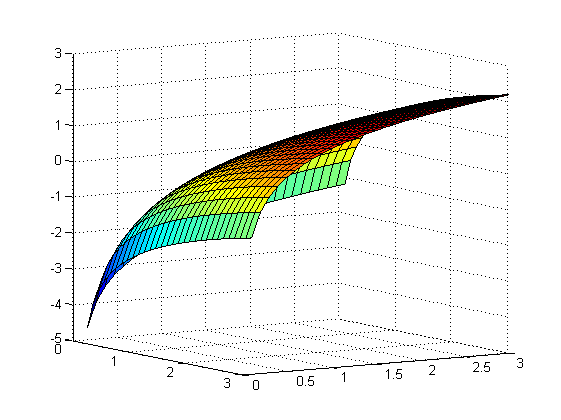
\includegraphics[width=0.66\textwidth]{logconsumption.png}
\end{figure}

\end{frame}

%%%%%%%%%%%%%%%%%%%%%%%%%%%%%%%%%%%%%%%%%%%%%%%
\begin{frame}{Multivariable Calculus}

\begin{figure}
\centering
\[f:\R^{2} \rightarrow \R \quad\quad f(K,L) = K^{\frac{1}{3}}L^{\frac{2}{3}}\]
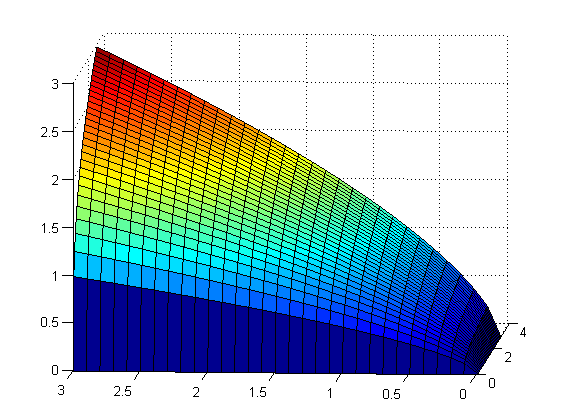
\includegraphics[width=0.66\textwidth]{cobbdouglas.png}
\end{figure}

\end{frame}

%%%%%%%%%%%%%%%%%%%%%%%%%%%%%%%%%%%%%%%%%%%%%%%
\begin{frame}{Level Sets}


A \bc{level set} of a function $f:\R^{n}\into \R$ is the set

\[ \mathcal{L} = \{\x \in \R^{n} \ | \ f(\x) = c  \} \]

for some $c \in \R$.\bigskip

Level sets for functions of two variables are often called \bc{level curves} or \bc{contours}. \bigskip

Familiar level sets from economics are the ``indifference curves'' of a utility function, the ``isoquants'' of a production function, and the ``iso-profit lines'' of a profit function.
\end{frame}


%%%%%%%%%%%%%%%%%%%%%%%%%%%%%%%%%%%%%%%%%%%%%%%
\begin{frame}{Level Sets}
\begin{figure}
\[ f:\R^{2}\rightarrow \R \quad\quad f(c_{1}, c_{2}) = \log c_{1} + \log c_{2}\]
	\begin{subfigure}[b]{0.45\textwidth}
		\centering
		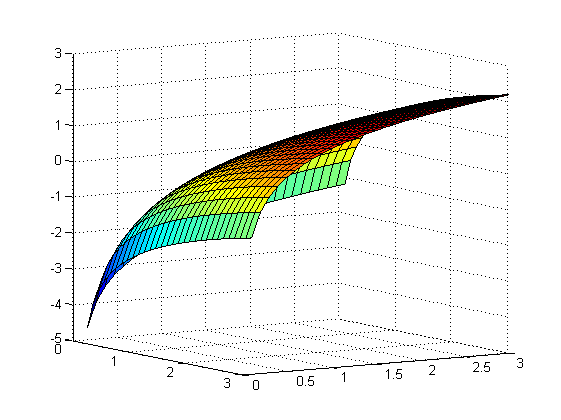
\includegraphics[width=\textwidth]{logconsumption.png}
		\caption{Surface}
	\end{subfigure}
	\begin{subfigure}[b]{0.45\textwidth}
		\centering
		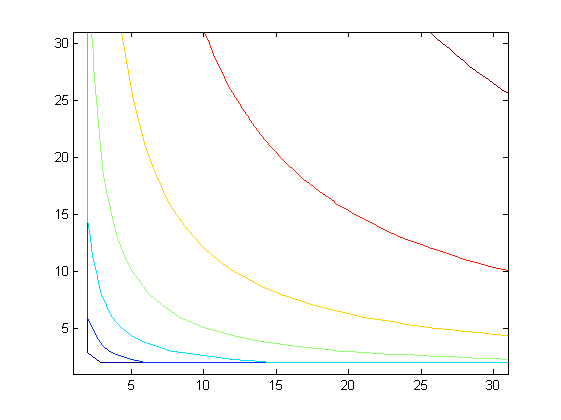
\includegraphics[width=\textwidth]{contour1.png}
		\caption{Contours}
	\end{subfigure}
\end{figure}

\vfill
\end{frame}

%%%%%%%%%%%%%%%%%%%%%%%%%%%%%%%%%%%%%%%%%%%%%%%
\begin{frame}{Partial Derivatives}

Derivatives tell us about the rate of change of a function. However, for functions of several variables, the rate of change may be different depending on what direction we wish to move.\bigskip

So let's look at the simple case where we're only changing one variable at a time. \bigskip 

The derivative when we only change one variable, keeping all others constant, is called the \bc{partial derivative}.  \bigskip
\end{frame}

%%%%%%%%%%%%%%%%%%%%%%%%%%%%%%%%%%%%%%%%%%%%%%%
\begin{frame}{Partial Derivatives}
Recall that the derivative of a function of one variable at some point $x_{0}$ is 

\[ \frac{df}{dx}(x_{0}) = \lim_{h\to 0} \frac{f(x_{0}+h) - f(x_{0})}{h} \]

\bigskip

The partial derivative of a function $f(x_{1}, x_{2},\dots,x_{n})$ with respect to $x_{i}$ at a point $\x^{0} = (x_{1}^{0}, x_{2}^{0},\dots,x_{n}^{0})$ is defined similarly.\bigskip



\[ \frac{\partial f}{\partial x_{i}} (x_{1}^{0}, x_{2}^{0},\dots,x_{n}^{0}) = \lim_{h\to 0} \frac{f(x_{1}^{0},\dots, x_{i}^{0} + h,\dots x_{n}^{0}) - f(x_{1}^{0},\dots, x_{i}^{0},\dots,x_{n}^{0})}{h}\]

\smallskip
if this limit exists.
\end{frame}
%%%%%%%%%%%%%%%%%%%%%%%%%%%%%%%%%%%%%%%%%%%%%%%
\begin{frame}{Partial Derivatives}
\begin{figure}
	\begin{subfigure}[b]{0.48\textwidth}
		\centering
		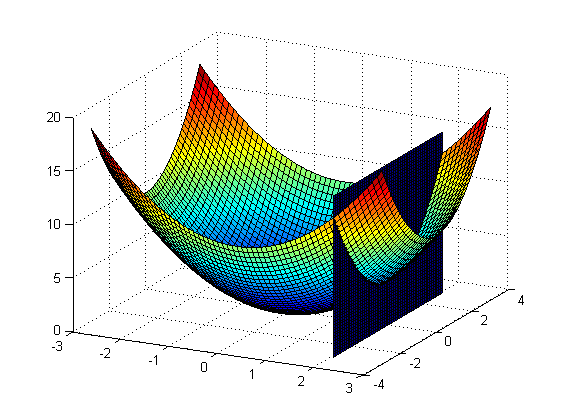
\includegraphics[width=\textwidth]{planeslice.png}
	\end{subfigure}
	\begin{subfigure}[b]{0.48\textwidth}
		\centering
		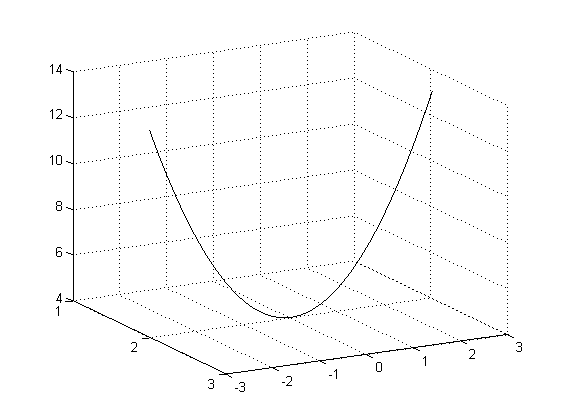
\includegraphics[width=\textwidth]{partial.png}
	\end{subfigure}
\end{figure}

\end{frame}

%%%%%%%%%%%%%%%%%%%%%%%%%%%%%%%%%%%%%%%%%%%%%%%
\begin{frame}{Chain Rules}

\begin{theorem}
Let $f\left(x_{1}(t),\dots,x_{n}(t)\right):\R^{n}\into\R$ be a differentiable function.

\[\frac{\mathrm{d}f}{\mathrm{d}t} = \frac{\partial f}{\partial x_{1}} \frac{\mathrm{d}x_{1}}{\mathrm{d} t} + \frac{\partial f}{\partial x_{2}}\frac{\mathrm{d}x_{2}}{\mathrm{d}t} + \dots + \frac{\partial f}{\partial x_{n}}\frac{\mathrm{d}x_{n}}{\mathrm{d}t}\]
\end{theorem}
\bigskip

\begin{theorem}
Let $f\left(x_{1}(u,v),\dots, x_{n}(u,v)\right):\R^{n}\into\R$ be a differentiable function

\[ \frac{\partial f}{\partial u} = \frac{\partial f}{\partial x_{1}}\frac{\partial x_{1}}{\partial u} + \frac{\partial f}{\partial x_{2}}\frac{\partial x_{2}}{\partial u} + \dots + \frac{\partial f}{\partial x_{n}}\frac{\partial x_{n}}{\partial u}\]
\end{theorem}

\end{frame}

%%%%%%%%%%%%%%%%%%%%%%%%%%%%%%%%%%%%%%%%%%%%%%%
\begin{frame}{Total Differential}

It is often useful to refer to the \bc{total differential}, which looks like the chain rule but using differentials rather than derivatives.

\[\mathrm{d}f = \frac{\partial f}{\partial x_{1}} \mathrm{d}x_{1} + \dots + \frac{\partial f}{\partial x_{n}} \mathrm{d}x_{n} \]

\end{frame}

%%%%%%%%%%%%%%%%%%%%%%%%%%%%%%%%%%%%%%%%%%%%%%%
\begin{frame}{Total Differential}

\begin{block}{Example}
For a function $f(x_{1}, x_{2}):\R^{2}\into\R$, find the slope of the tangent to a level curve of $f$ (assuming $f_{x_{2}} \not = 0$).\\

Recall that a level curve sets the function to a constant level
\[f(x_{1},x_{2}) = k\]
Now totally differentiate both sides

\begin{align*}
&f_{x_{1}} \mathrm{d}x_{1} + f_{x_{2}} \mathrm{d}x_{2} = 0\\
&f_{x_{2}} \mathrm{d}x_{2} = -f_{x_{1}} \mathrm{d}x_{1}\\
& \frac{\mathrm{d}x_{2}}{\mathrm{d}x_{1}} = - \frac{f_{x_{1}}}{f_{x_{2}}}
\end{align*}

\end{block}
\end{frame}

%%%%%%%%%%%%%%%%%%%%%%%%%%%%%%%%%%%%%%%%%%%%%%%
\begin{frame}{Gradient}

The \bc{gradient} is a vector containing all the first partial derivatives. The gradient vector is written interchangeably as $Df(\x)$ or $\nabla f(\x)$.\bigskip

Let $f:\R^{n} \into \R$.

\[\nabla f(\x) = \left (\frac{\partial f}{\partial x_{1}}, \frac{\partial f}{\partial x_{2}},\dots, \frac{\partial f}{\partial x_{n}}   \right ) \]
\bigskip 

\begin{exercise}
Let $f:\R^{3} \into \R$ and $f(x,y,z) = x^{2} + xyz + y^{2} - z^{3}$. Find the gradient.
\end{exercise}
\end{frame}

%%%%%%%%%%%%%%%%%%%%%%%%%%%%%%%%%%%%%%%%%%%%%%%
\begin{frame}{Gradient}

\begin{block}{Proposition}
Let $f:\R^{2} \into \R$ and let $\x$ be a regular point of $f$, then the tangent to the level curve at $\x$ is orthogonal to the gradient at $\x$.
\end{block}
\begin{exercise}\textit{Proof:}
\end{exercise}
\bigskip\vfill\vfill
\end{frame}

%%%%%%%%%%%%%%%%%%%%%%%%%%%%%%%%%%%%%%%%%%%%%%%
\begin{frame}{Directional Derivative}

Let $f:\R^{n}\into\R$ be a $\mathcal{C}^{1}$ function on a ball about $\x$. \bigskip

Let $\v \in \R^{n}$ be a unit vector.\bigskip

 The derivative of $f$ at $\x$ in the direction $\v$ is
\[D_{v}f(\x) = \nabla f(\x) \cdot \v\]
\vfill\vfill
\end{frame}
%%%%%%%%%%%%%%%%%%%%%%%%%%%%%%%%%%%%%%%%%%%%%%%
\begin{frame}{Directional Derivative}

 Recall that
\[a \cdot b = ||a|| \, ||b|| \, \cos \theta\]
\bigskip

The rate of increase in some direction $\v$ at a point $\x$ is

\[D_{\v}f(\x) = \nabla f(\x)\cdot \v = ||\nabla f(\x)|| \, ||\v||\, \cos \theta\]
\medskip

Recall that $-1 \leq \cos \theta \leq 1$. Since the length of $\v$ is fixed at unity, the derivative is maximised by choosing a $\v$ such that $\cos \theta = 1$.\bigskip

 This occurs when the angle between $\v$ and the gradient is $\theta = 0$, or when $\v$ points in the same direction as $\nabla f(\x)$.\\
\end{frame}
%%%%%%%%%%%%%%%%%%%%%%%%%%%%%%%%%%%%%%%%%%%%%%%
\begin{frame}{The Hessian}
Similar to how the gradient is a vector containing all the first order partials of a function, we may want to consider a matrix full of the second order partials. This is called the \bc{Hessian} matrix and is written $D^{2}f(\x)$.\bigskip


Let $f:\R^{n}\into\R$ be a twice differentiable function. The Hessian is
\large
\[D^{2}f = 
\begin{pmatrix}
\frac{\partial^{2}f}{\partial x_{1}^{2}} & \frac{\partial^{2} f}{\partial x_{2}\partial x_{1}} & \dots & \frac{\partial^{2} f}{\partial x_{n} \partial x_{1}}\\
\frac{\partial^{2} f}{\partial x_{1}\partial x_{2}} & \frac{\partial^{2} f}{\partial x_{2}^{2}} & \dots & \frac{\partial^{2} f}{\partial x_{n}\partial x_{2}}\\
\vdots & \vdots & \ddots & \vdots\\
\frac{\partial^{2} f}{\partial x_{1} \partial x_{n}} & \frac{\partial^{2} f}{\partial x_{2} \partial x_{n}} & \dots & \frac{\partial^{2} f}{\partial x_{n}^{2}}
\end{pmatrix}
\]
\normalsize
\medskip

Note that if $f$ is a twice \emph{continuously} differentiable function, the Hessian will be a symmetric matrix.


\end{frame}

%%%%%%%%%%%%%%%%%%%%%%%%%%%%%%%%%%%%%%%%%%%%%%%
\begin{frame}{Taylor Series in $\R^{n}$}

\begin{theorem}
Let $F$ be a $\mathcal{C}^{2}$ function defined on an open ball in $\R^{n}$. For any point $\a$ in the ball there exists a $\mathcal{C}^{2}$ function $R_{2}(\h;\a)$ such that for any point $\a + \h$ in the ball

\[F(\a + \h) = F(\a) + DF(\a) \h + \frac{1}{2}\h^{T}D^{2}F(\a)\h + R_{2}(\h;\a)\]

where

\[ \frac{R_{2}(\h;\a)}{||\h||^{2}} \rightarrow 0 \text{  as  } \h \rightarrow 0\]
\end{theorem}
\bigskip

The key difference between Taylor expansions for single variable vs multivariable functions is that a multivariable expansion isn't just a function of the first $k$ derivatives, but is also a function of the \emph{cross partials}.
\vfill\vfill

\end{frame}

%%%%%%%%%%%%%%%%%%%%%%%%%%%%%%%%%%%%%%%%%%%%%%%
\begin{frame}{Steady State}

As we'll see in the coming lectures, our optimization problems will yield a description of a dynamic system.\bigskip

For example, the Solow growth model assumes a production function that uses capital, $F(k_{t})$, a constant savings rate $s$, and a capital depreciation rate $\delta$.

\[k_{t+1} = sF(k_{t}) + (1-\delta) k_{t}\]

Some dynamic models admit a \bc{steady state}, where the variables become time invariant.

\[\bar{k} = sF(\bar{k}) + (1-\delta)\bar{k}\]

\end{frame}

%%%%%%%%%%%%%%%%%%%%%%%%%%%%%%%%%%%%%%%%%%%%%%%
\begin{frame}{Log-linearization}

In log-linearizing an equation, we want to transform it from being in levels to being in percentage deviation from the steady state

\[\hat{x}_{t} = \frac{x_{t} - \bar{x}}{\bar{x}}\]
\bigskip

For most equations, we won't be able to write it like this exactly. We'll need to write it approximately:

\begin{align*}
f(x_{t}) &\approx f(\bar{x}) + f^{\prime}(\bar{x}) (x_{t} - \bar{x})\\
&= f(\bar{x}) + f^{\prime}(\bar{x})\bar{x} \hat{x}_{t}
\end{align*}
\end{frame}

%%%%%%%%%%%%%%%%%%%%%%%%%%%%%%%%%%%%%%%%%%%%%%%
\begin{frame}{Log-linearization}

We can do the same Taylor expansion for multivariable functions:

\begin{align*}
f(x_{t}, y_{t}) &\approx f(\bar{x}, \bar{y}) + f_{x}(\bar{x}, \bar{y})(x_{t} - \bar{x}) + f_{y}(\bar{x}, \bar{y})(y_{t} - \bar{y})\\
& = f(\bar{x}, \bar{y}) + f_{x}(\bar{x}, \bar{y})\bar{x}\hat{x}_{t} + f_{y}(\bar{x}, \bar{y})\bar{y}\hat{y}_{t}
\end{align*}

\end{frame}

%%%%%%%%%%%%%%%%%%%%%%%%%%%%%%%%%%%%%%%%%%%%%%%
\begin{frame}{Log-linearization}
\begin{exercise}
Log-linearize the following equations around their steady state:
\begin{enumerate}
	\item $Y_{t} = C_{t} + I_{t}$
	\item $k_{t+1} = sk_{t}^{\alpha} + (1-\delta)k_{t}$
\end{enumerate}
\end{exercise}
\bigskip\vfill\vfill
\end{frame}

%%%%%%%%%%%%%%%%%%%%%%%%%%%%%%%%%%%%%%%%%%%%%%%
\begin{frame}{Log-linearization}

\begin{figure}
	\centering
	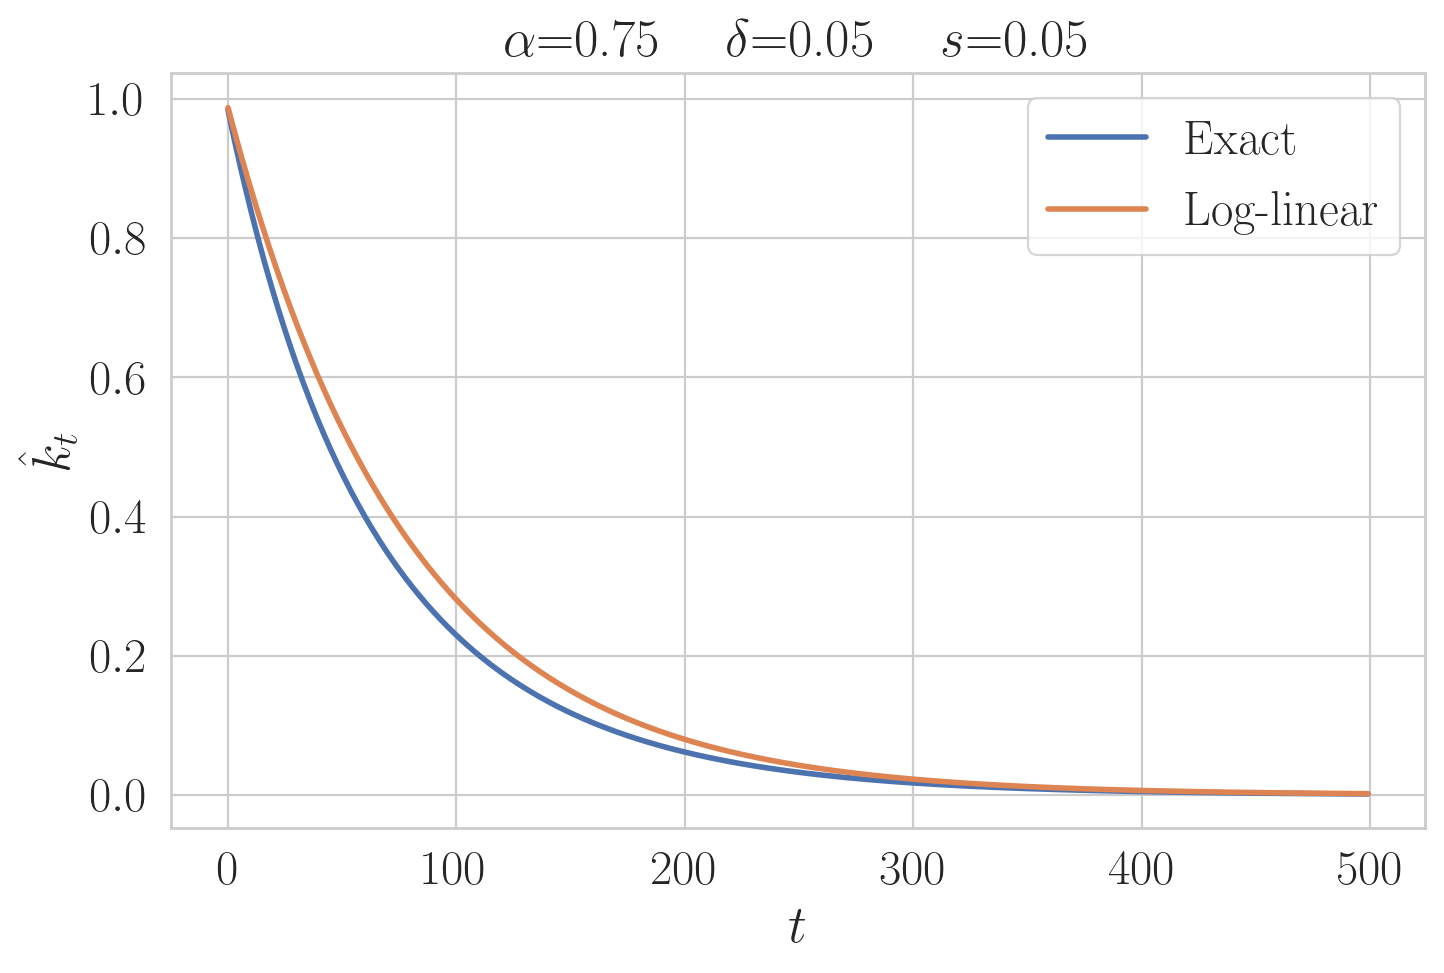
\includegraphics[width=0.75\textwidth]{solow.png}
	\caption{Solow model: Exact vs Log-linearized}
\end{figure}
\end{frame}
%%%%%%%%%%%%%%%%%%%%%%%%%%%%%%%%%%%%%%%%%%%%%%%
\begin{frame}{Learning Outcomes}

\bc{You should be able to:}
\begin{itemize}
	\item Expand a function into its Taylor series.
	\item Verify first order necessary and second order sufficient conditions for univariate functions.
	\item Take partial derivatives.
	\item Construct the gradient vector.	
	\item Construct the Hessian.
	\item Log-linearize an equation.
\end{itemize}

\end{frame}
\end{document}	